\begin{figure}
\centering
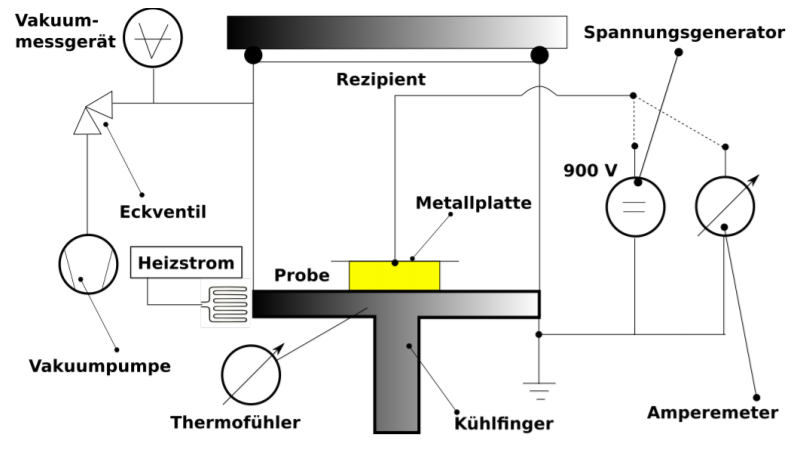
\includegraphics[width=0.7\textwidth]{aufbau.png}
\caption{Schematische Darstellung des Versuchaufbaus \cite[3]{anleitung}.}
\label{fig:aufbau}
\end{figure}

Der Kaliumbromid-Kristall ist mit Strontium dotiert. Während der Messung befindet sich der Kristall in einem Behälter der mit einer Vakuumpumpe
verbunden ist. Dabei sollte das Vakuum etwa $10^{-2}$ mb betragen.

Auf der Probe sowie auf dem Boden des Behälters liegt jeweils eine Metallplatte, sodass sich ein Plattenkodensator
ergibt. An diesen kann über einen Spannungsgenerator ein elektrisches Feld angelegt werden.

Am Boden des Behälters befindet sich außerdem noch eine Heizstromquelle sowie ein Kühlfinger der in flüssiges Stickstoff
getaucht ist. So kann die Probe aufgewärmt oder abgekühlt werden. Über ein Thermoelement kann die entsprechende Temperatur
abgelesen werden.

Um den Strom ablesen zu können, wird noch ein Picoamperemeter angeschlossen.
